% Options for packages loaded elsewhere
\PassOptionsToPackage{unicode}{hyperref}
\PassOptionsToPackage{hyphens}{url}
%
\documentclass[
  12pt,
]{article}
\usepackage{amsmath,amssymb}
\usepackage{iftex}
\ifPDFTeX
  \usepackage[T1]{fontenc}
  \usepackage[utf8]{inputenc}
  \usepackage{textcomp} % provide euro and other symbols
\else % if luatex or xetex
  \usepackage{unicode-math} % this also loads fontspec
  \defaultfontfeatures{Scale=MatchLowercase}
  \defaultfontfeatures[\rmfamily]{Ligatures=TeX,Scale=1}
\fi
\usepackage{lmodern}
\ifPDFTeX\else
  % xetex/luatex font selection
    \setmainfont[]{Times New Roman}
\fi
% Use upquote if available, for straight quotes in verbatim environments
\IfFileExists{upquote.sty}{\usepackage{upquote}}{}
\IfFileExists{microtype.sty}{% use microtype if available
  \usepackage[]{microtype}
  \UseMicrotypeSet[protrusion]{basicmath} % disable protrusion for tt fonts
}{}
\makeatletter
\@ifundefined{KOMAClassName}{% if non-KOMA class
  \IfFileExists{parskip.sty}{%
    \usepackage{parskip}
  }{% else
    \setlength{\parindent}{0pt}
    \setlength{\parskip}{6pt plus 2pt minus 1pt}}
}{% if KOMA class
  \KOMAoptions{parskip=half}}
\makeatother
\usepackage{xcolor}
\usepackage[margin=1in]{geometry}
\usepackage{color}
\usepackage{fancyvrb}
\newcommand{\VerbBar}{|}
\newcommand{\VERB}{\Verb[commandchars=\\\{\}]}
\DefineVerbatimEnvironment{Highlighting}{Verbatim}{commandchars=\\\{\}}
% Add ',fontsize=\small' for more characters per line
\usepackage{framed}
\definecolor{shadecolor}{RGB}{248,248,248}
\newenvironment{Shaded}{\begin{snugshade}}{\end{snugshade}}
\newcommand{\AlertTok}[1]{\textcolor[rgb]{0.94,0.16,0.16}{#1}}
\newcommand{\AnnotationTok}[1]{\textcolor[rgb]{0.56,0.35,0.01}{\textbf{\textit{#1}}}}
\newcommand{\AttributeTok}[1]{\textcolor[rgb]{0.13,0.29,0.53}{#1}}
\newcommand{\BaseNTok}[1]{\textcolor[rgb]{0.00,0.00,0.81}{#1}}
\newcommand{\BuiltInTok}[1]{#1}
\newcommand{\CharTok}[1]{\textcolor[rgb]{0.31,0.60,0.02}{#1}}
\newcommand{\CommentTok}[1]{\textcolor[rgb]{0.56,0.35,0.01}{\textit{#1}}}
\newcommand{\CommentVarTok}[1]{\textcolor[rgb]{0.56,0.35,0.01}{\textbf{\textit{#1}}}}
\newcommand{\ConstantTok}[1]{\textcolor[rgb]{0.56,0.35,0.01}{#1}}
\newcommand{\ControlFlowTok}[1]{\textcolor[rgb]{0.13,0.29,0.53}{\textbf{#1}}}
\newcommand{\DataTypeTok}[1]{\textcolor[rgb]{0.13,0.29,0.53}{#1}}
\newcommand{\DecValTok}[1]{\textcolor[rgb]{0.00,0.00,0.81}{#1}}
\newcommand{\DocumentationTok}[1]{\textcolor[rgb]{0.56,0.35,0.01}{\textbf{\textit{#1}}}}
\newcommand{\ErrorTok}[1]{\textcolor[rgb]{0.64,0.00,0.00}{\textbf{#1}}}
\newcommand{\ExtensionTok}[1]{#1}
\newcommand{\FloatTok}[1]{\textcolor[rgb]{0.00,0.00,0.81}{#1}}
\newcommand{\FunctionTok}[1]{\textcolor[rgb]{0.13,0.29,0.53}{\textbf{#1}}}
\newcommand{\ImportTok}[1]{#1}
\newcommand{\InformationTok}[1]{\textcolor[rgb]{0.56,0.35,0.01}{\textbf{\textit{#1}}}}
\newcommand{\KeywordTok}[1]{\textcolor[rgb]{0.13,0.29,0.53}{\textbf{#1}}}
\newcommand{\NormalTok}[1]{#1}
\newcommand{\OperatorTok}[1]{\textcolor[rgb]{0.81,0.36,0.00}{\textbf{#1}}}
\newcommand{\OtherTok}[1]{\textcolor[rgb]{0.56,0.35,0.01}{#1}}
\newcommand{\PreprocessorTok}[1]{\textcolor[rgb]{0.56,0.35,0.01}{\textit{#1}}}
\newcommand{\RegionMarkerTok}[1]{#1}
\newcommand{\SpecialCharTok}[1]{\textcolor[rgb]{0.81,0.36,0.00}{\textbf{#1}}}
\newcommand{\SpecialStringTok}[1]{\textcolor[rgb]{0.31,0.60,0.02}{#1}}
\newcommand{\StringTok}[1]{\textcolor[rgb]{0.31,0.60,0.02}{#1}}
\newcommand{\VariableTok}[1]{\textcolor[rgb]{0.00,0.00,0.00}{#1}}
\newcommand{\VerbatimStringTok}[1]{\textcolor[rgb]{0.31,0.60,0.02}{#1}}
\newcommand{\WarningTok}[1]{\textcolor[rgb]{0.56,0.35,0.01}{\textbf{\textit{#1}}}}
\usepackage{longtable,booktabs,array}
\usepackage{calc} % for calculating minipage widths
% Correct order of tables after \paragraph or \subparagraph
\usepackage{etoolbox}
\makeatletter
\patchcmd\longtable{\par}{\if@noskipsec\mbox{}\fi\par}{}{}
\makeatother
% Allow footnotes in longtable head/foot
\IfFileExists{footnotehyper.sty}{\usepackage{footnotehyper}}{\usepackage{footnote}}
\makesavenoteenv{longtable}
\usepackage{graphicx}
\makeatletter
\def\maxwidth{\ifdim\Gin@nat@width>\linewidth\linewidth\else\Gin@nat@width\fi}
\def\maxheight{\ifdim\Gin@nat@height>\textheight\textheight\else\Gin@nat@height\fi}
\makeatother
% Scale images if necessary, so that they will not overflow the page
% margins by default, and it is still possible to overwrite the defaults
% using explicit options in \includegraphics[width, height, ...]{}
\setkeys{Gin}{width=\maxwidth,height=\maxheight,keepaspectratio}
% Set default figure placement to htbp
\makeatletter
\def\fps@figure{htbp}
\makeatother
\setlength{\emergencystretch}{3em} % prevent overfull lines
\providecommand{\tightlist}{%
  \setlength{\itemsep}{0pt}\setlength{\parskip}{0pt}}
\setcounter{secnumdepth}{5}
% definitions for citeproc citations
\NewDocumentCommand\citeproctext{}{}
\NewDocumentCommand\citeproc{mm}{%
  \begingroup\def\citeproctext{#2}\cite{#1}\endgroup}
\makeatletter
 % allow citations to break across lines
 \let\@cite@ofmt\@firstofone
 % avoid brackets around text for \cite:
 \def\@biblabel#1{}
 \def\@cite#1#2{{#1\if@tempswa , #2\fi}}
\makeatother
\newlength{\cslhangindent}
\setlength{\cslhangindent}{1.5em}
\newlength{\csllabelwidth}
\setlength{\csllabelwidth}{3em}
\newenvironment{CSLReferences}[2] % #1 hanging-indent, #2 entry-spacing
 {\begin{list}{}{%
  \setlength{\itemindent}{0pt}
  \setlength{\leftmargin}{0pt}
  \setlength{\parsep}{0pt}
  % turn on hanging indent if param 1 is 1
  \ifodd #1
   \setlength{\leftmargin}{\cslhangindent}
   \setlength{\itemindent}{-1\cslhangindent}
  \fi
  % set entry spacing
  \setlength{\itemsep}{#2\baselineskip}}}
 {\end{list}}
\usepackage{calc}
\newcommand{\CSLBlock}[1]{\hfill\break\parbox[t]{\linewidth}{\strut\ignorespaces#1\strut}}
\newcommand{\CSLLeftMargin}[1]{\parbox[t]{\csllabelwidth}{\strut#1\strut}}
\newcommand{\CSLRightInline}[1]{\parbox[t]{\linewidth - \csllabelwidth}{\strut#1\strut}}
\newcommand{\CSLIndent}[1]{\hspace{\cslhangindent}#1}
\usepackage{tcolorbox}
\usepackage{amssymb}
\usepackage{yfonts}
\usepackage{bm}
\usepackage{titlesec}
\usepackage{kbordermatrix}


\newtcolorbox{greybox}{
  colback=white,
  colframe=blue,
  coltext=black,
  boxsep=5pt,
  arc=4pt}
  
\newcommand{\sectionbreak}{\clearpage}

 
\newcommand{\ds}[4]{\sum_{{#1}=1}^{#3}\sum_{{#2}=1}^{#4}}
\newcommand{\us}[3]{\mathop{\sum\sum}_{1\leq{#2}<{#1}\leq{#3}}}

\newcommand{\ol}[1]{\overline{#1}}
\newcommand{\ul}[1]{\underline{#1}}

\newcommand{\amin}[1]{\mathop{\text{argmin}}_{#1}}
\newcommand{\amax}[1]{\mathop{\text{argmax}}_{#1}}

\newcommand{\ci}{\perp\!\!\!\perp}

\newcommand{\mc}[1]{\mathcal{#1}}
\newcommand{\mb}[1]{\mathbb{#1}}
\newcommand{\mf}[1]{\mathfrak{#1}}

\newcommand{\eps}{\epsilon}
\newcommand{\lbd}{\lambda}
\newcommand{\alp}{\alpha}
\newcommand{\df}{=:}
\newcommand{\am}[1]{\mathop{\text{argmin}}_{#1}}
\newcommand{\ls}[2]{\mathop{\sum\sum}_{#1}^{#2}}
\newcommand{\ijs}{\mathop{\sum\sum}_{1\leq i<j\leq n}}
\newcommand{\jis}{\mathop{\sum\sum}_{1\leq j<i\leq n}}
\newcommand{\sij}{\sum_{i=1}^n\sum_{j=1}^n}
	
\ifLuaTeX
  \usepackage{selnolig}  % disable illegal ligatures
\fi
\usepackage{bookmark}
\IfFileExists{xurl.sty}{\usepackage{xurl}}{} % add URL line breaks if available
\urlstyle{same}
\hypersetup{
  pdfauthor={Jan de Leeuw - University of California Los Angeles},
  hidelinks,
  pdfcreator={LaTeX via pandoc}}

\title{Smacof at 50: A Manual\\
Part 2: Metric Smacof}
\author{Jan de Leeuw - University of California Los Angeles}
\date{Started December 12 2022, Version of May 03, 2024}

\begin{document}
\maketitle
\begin{abstract}
TBD
\end{abstract}

{
\setcounter{tocdepth}{3}
\tableofcontents
}
\textbf{Note:} This is a working manuscript which will be expanded/updated
frequently. All suggestions for improvement are welcome. All Rmd, tex,
html, pdf, R, and C files are in the public domain. Attribution will be
appreciated, but is not required. All files can be found at
\url{https://github.com/deleeuw} in the repositories smacofCode, smacofManual,
and smacofExamples. A barebones R package is in the repository
smacofAC.

\section{Introduction}\label{introduction}

In this part of the manual we discuss metric MDS, and the program
smacofAC. Metric MDS is the core of all smacof programs, because they
all have the majorization basec on the Guttman transform in common.

\section{Bells and Whistles}\label{bells-and-whistles}

There are two options, \emph{bounds} and \emph{constant}, to make smacofAC more interesting and more widely applicable. Using these options the metric MDS problem becomes minimization of
\[
\sigma(X,\hat D)=\sum\sum w_{ij}(\hat d_{ij}-d_{ij}(X))^2
\]
over both \(X\) and \(\hat D\), allowing some limited ``metric'' transformations of the data \(\Delta\).
The four ``metric'' types of transformations are

\begin{enumerate}
\def\labelenumi{\arabic{enumi}.}
\tightlist
\item
  type AC1: if bounds = 0 and constant = 0 \(\hat d_{ij}=\delta_{ij}\).
\item
  type AC2: if bounds = 0 and constant = 1 \(\hat d_{ij}=\delta_{ij}+c\) for some \(c\),
\item
  type AC3: if bounds = 1 and constant = 0 \(\delta^-_{ij}\leq\hat d_{ij}\leq\delta^+_{ij}\),
\item
  type AC4: if bounds = 1 and constant = 1 \(\delta^-_{ij}+c\leq\hat d_{ij}\leq\delta^+_{ij}+c\) for some \(c\),
\end{enumerate}

Here \(\Delta^-\) and \(\Delta^+\) are known matrices with bounds, and \(c\) is the unknown additive constant. All four types of transformations also require that \(\hat d_{ij}\geq 0\) for all \((i,j)\). There are extensions of the smacof theory (Heiser (1991)) that do not require non-negativity of the disparities, but in the implementations in this manual we always force
them to be non-negative. Note that AC3 is AC4 with \(c=0\) and AC2 is AC4 with \(\Delta^-=\Delta^+=\Delta\).

Note that for types AC2 and AC4 the data \(\Delta\) do not need to be non-negative. In fact,
the original motivation for the additive constant in classical scaling (Messick and Abelson (1956))
was that Thurstonian analysis of paired or triadic comparisons produced dissimilarities on an interval scale, and thus could very well include negative values.

In AC3 and AC4 there is no mention of \(\Delta\), which means
the bounds \(\Delta^-\) and \(\Delta^+\) are actually the data. We could
collect dissimilarity data by asking subjects for interval judgments. Instead
of a rating scale with possible responses from one to ten we could ask
for a mark on a line between zero and ten, and then interpret the
marks as a choice of one of the intervals \([k, k+1]\). These finite precision
or interval type of data could even come from physical measurements of distances.
Thus the bounds parameter provides one way to incorporate uncertainty into MDS, similar to interval analysis, fuzzy computing, or soft computing.

The non-negativity requirement for \(\hat D\) implies bounds for the additive constant
\(c\). In AC2 we need \(c\geq-\min\delta_{ij}\) to maintain non-negativity. For AC4 we must have \(c\geq-\min\delta_{ij}^+\), otherwise the constraints on the transformation are inconsistent.
Clearly for consistency of AC3 and AC4 we require that \(\delta_{ij}^-\leq\delta_{ij}^+\)
for all \((i,j)\). It makes sense in most situations to choose \(\Delta^-\) and \(\Delta^+\)
to be monotone with \(\Delta\), but there is no requirement to do so.

\section{Implementation}\label{implementation}

\subsection{Type AC1}\label{type-ac1}

This is standard non-metric smacof, no bells and whistles. The user has to make some choices,
coded in the parameter file.

\begin{Shaded}
\begin{Highlighting}[]
\NormalTok{nobj   }\DecValTok{9}
\NormalTok{ndim   }\DecValTok{2}
\NormalTok{init   }\DecValTok{2}
\NormalTok{width   }\DecValTok{10}
\NormalTok{precision   }\DecValTok{6}
\NormalTok{haveweights   }\DecValTok{0}
\NormalTok{havelabels }\DecValTok{1}
\NormalTok{itmax   }\DecValTok{10000}
\NormalTok{epsi   }\DecValTok{10}
\NormalTok{verbose   }\DecValTok{1}
\NormalTok{kitmax   }\DecValTok{1}
\NormalTok{kepsi   }\DecValTok{1}
\NormalTok{kverbose   }\DecValTok{0}
\NormalTok{constant }\DecValTok{1}
\NormalTok{bounds }\DecValTok{1}
\NormalTok{alpha }\DecValTok{10}
\end{Highlighting}
\end{Shaded}

The parameters \emph{constant}, \emph{bounds}, \emph{alpha}, \emph{kitmax}, \emph{kepsi}, and \emph{kverbose} are only relevant for AC2, AC3, and AC4. Nevertheless even for AC1 they should have integer values, it just doesn't matter what these values are.
Parameter \emph{ndim} is the number of dimensions, and \emph{init} tells if an initial configuration
is read from a file (init = 1), is computed using classical scaling (init = 2), or is
a random configuration (init = 3). If \emph{haveweights} is one a vector of weights is read from a file, of \emph{labels} is one a vector of labels for the configuration plot is read in. Parameters
\emph{itmax}, \emph{epsi}, and \emph{verbose} control the iterations. The maximum number of iterations
is \emph{itmax}, the iterations stop if the decrease of stress in an iteration is less than
1E-\emph{epsi}, and if \emph{verbose} is one intermediate iteration results are written to stdout.
These intermediate iteration results are formatted with the R function formatC(), using
\emph{width} for the width argument and \emph{precision} for the digits argument.

\subsection{Type AC2}\label{type-ac2}

For AC2 we also optimize over the additive constant \(c\), and thus the ALS algorithm has two
sub-steps. The first sub-step consists of a number of Guttman iterations to update \(X\) for given
\(\hat D\) (i.e.~for given \(c\)) and the second sub-step updates \(c\) for given \(X\).
Parameters \emph{kitmax}, \emph{kepsi}, and \emph{kverbose} control the inner iterations in the first sub-step in the same way as \emph{itmax}, \emph{epsi}, and \emph{verbose} control the
outer iterations that include both sub-steps. No inner iterations are used
to update the additive constant, which only requires computing the weighted
average.
\begin{equation}
c=-\frac{\sum\sum w_{ij}(\delta_{ij}-d_{ij}(X))}{\sum\sum w_{ij}}
\label{eq:updac2}
\end{equation}
AC2 should give the same results as the technique of Cooper (1972).

\subsection{Type AC3}\label{type-ac3}

The algorithm for AC3 has the same structure as that for AC2. Instead of
a second sub-step computing the additive constant, the second sub-step
computes \(\hat D\) by squeezing the \(D(X)\) into the bounds. Thus
\begin{equation}
\hat d_{ij}=\begin{cases}
\delta_{ij}^-&\text{ if }d_{ij}(X)<\delta_{ij}^-,\\
\delta_{ij}^+&\text{ if }d_{ij}(X)>\delta_{ij}^+,\\
d_{ij}(X)&\text{ otherwise }.
\end{cases}
\label{eq:updac3}
\end{equation}
Obviously no iterations are required in the second sub-step.

For AC3 the parameter \emph{alpha} may also be relevant. If the \emph{bounds} parameter
is equal to one then \(\Delta^-\) and \(\Delta^+\) are read from a file (as vectors with the lower diagonal elements in row-major order, as is the case for \(\Delta\) and \(W\)). If \emph{bounds}
is two we set
\begin{subequations}
\begin{align}
\delta_{ij}^-&=\delta_{ij}-\frac{\text{range}(\Delta)}{\alpha},\\
\delta_{ij}^+&=\delta_{ij}+\frac{\text{range}(\Delta)}{\alpha},
\end{align}
\end{subequations}
and if \emph{bounds} is three we set
\begin{subequations}
\begin{align}
\delta_{ij}^-&=(1-\frac{1}{\alpha})\delta_{ij},\\
\delta_{ij}^+&=(1+\frac{1}{\alpha})\delta_{ij}.
\end{align}
\end{subequations}
In keeping with the general smacof conventions for parameters we use an integer
parameter for \(\alpha\).

\subsection{Type AC4}\label{type-ac4}

Of the four regression problems in the second ALS sub-step only the one for AC4 with both bounds and additive constant is non-trivial. We'll give it some extra attention.

It may help to give an example of what it actually requires. We use the De Gruijter example
with nine Dutch political parties from 1967 (De Gruijter (1967)). For ease of reference we include the data here. Dissimilarities are averages over a group of 100 introductory psychology students.

\begin{verbatim}
##       KVP PvdA  VVD  ARP  CHU  CPN  PSP   BP
## PvdA 5.63                                   
## VVD  5.27 6.72                              
## ARP  4.60 5.64 5.46                         
## CHU  4.80 6.22 4.97 3.20                    
## CPN  7.54 5.12 8.13 7.84 7.80               
## PSP  6.73 4.59 7.55 6.73 7.08 4.08          
## BP   7.18 7.22 6.90 7.28 6.96 6.34 6.88     
## D66  6.17 5.47 4.67 6.13 6.04 7.42 6.36 7.36
\end{verbatim}

We compute distances from the Torgerson solution. The Shepard plot for \(c=0\) and the Torgerson distances is in figure \ref{fig:bandplot}. The two blue
lines are connecting the \(\delta_{ij}^-\) and the \(\delta_{ij}^+\), i.e.~they give
the bounds for \(c=0\). In our example the lines are parallel, because \(\delta_{ij}^+-\delta_{ij}^-=2\) for all \((i,j)\), but in general this may not be the case.
The points between the two lines do not contribute to the loss, and
the points outside the band contribute by how much they are outside, as indicated by the
black vertical lines.

\begin{figure}

{\centering 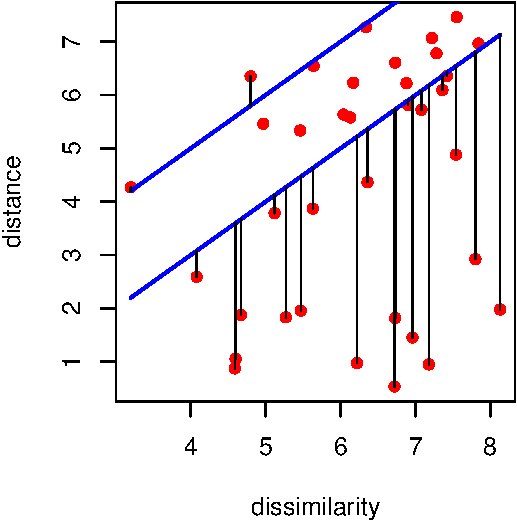
\includegraphics{smacofAC_files/figure-latex/bandplot-1} 

}

\caption{De Gruijter Shepard Plot}\label{fig:bandplot}
\end{figure}

By varying \(c\) we shift the region between the two parallel lines upwards or downwards. The width of the region, or more generally the shape, always remains the same, because it is determined by the difference of \(\delta^+\) and \(\delta^-\) and does not depend on \(c\). The
optimal \(c\) is that shift for which the red \((\delta_{ij},d_{ij}(X))\) points are as much as possible within the strip between the \(\delta^-\) and \(\delta^+\) lines. This is in the least squares sense, which means that we minimize the horizontal squared distances from the points outside the strip to the \(\delta^-\) and \(\delta^+\) lines (i.e.~the black vertical lines).

Let's formalize this. Define
\begin{equation}
\phi_{ij}(c):=\min_{\delta_{ij}\geq 0}\{(\delta_{ij}-d_{ij}(X))^2\mid \delta^-_{ij}+c\leq\delta_{ij}\leq\delta^+_{ij}+c\}
\label{eq:phiijdef}
\end{equation}
and
\begin{equation}
\phi(c):=\sum\sum w_{ij}\phi_{ij}(c)
\label{eq:phidef}
\end{equation}
The constraints are consistent if \(\delta_{ij}^++c\geq 0\), i.e.~if \(c\geq c_0:=-\min\delta_{ij}^+\).
The regression problem is to minimize \(\phi\) over \(c\geq c_0:=-\min\delta_{ij}^+\).

Figure \ref{fig:onefunc} has an example of one of the \(\phi_{ij}\). The value of the
\(d_{ij}(X)\) we used is 4.2698418, \(\delta_{ij}\) is 3.2, \(\delta_{ij}^-\) is 2.2, and \(\delta_{ij}^+\) is 4.2.
The two red vertical lines
are at \(c=d_{ij}(X)-\delta_{ij}^+\) and \(c=d_{ij}(X)-\delta_{ij}^-\).

Now
\begin{equation}
\hat d_{ij}=\begin{cases}
\delta_{ij}^-+c&\text{ if }c\geq d_{ij}(X)-\delta_{ij}^-,\\
\delta_{ij}^++c&\text{ if }c\leq d_{ij}(X)-\delta_{ij}^+,\\
d_{ij}(X)&\text{ otherwise}.
\end{cases}
\label{eq:solves}
\end{equation}
and thus
\begin{equation}
\phi_{ij}(c)=\begin{cases}
(d_{ij}(X)-(\delta_{ij}^-+c))^2&\text{ if }c\geq d_{ij}(X)-\delta_{ij}^-,\\
(d_{ij}(X)-(\delta_{ij}^++c))^2&\text{ if }c\leq d_{ij}(X)-\delta_{ij}^+,\\
0&\text{ otherwise}.
\end{cases}
\label{eq:funcs}
\end{equation}
It follows that \(\phi_{ij}\) is
piecewise quadratic, convex, and continuously differentiable. The derivative
is piecewise linear, continuous, and increasing. In fact
\begin{equation}
\mathcal{D}\phi_{ij}(c)=\begin{cases}
2(c-(d_{ij}(X)-\delta_{ij}^-))&\text{ if }c\geq d_{ij}(X)-\delta_{ij}^-,\\
2(c-(d_{ij}(X)-\delta_{ij}^+))&\text{ if }c\leq d_{ij}(X)-\delta_{ij}^+,\\
0&\text{ otherwise}.
\end{cases}
\label{eq:derivs}
\end{equation}

\begin{figure}
\centering
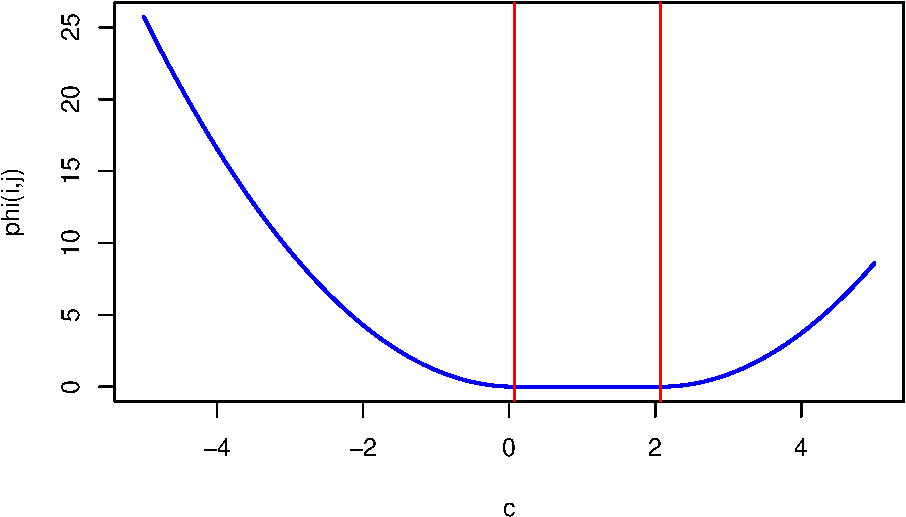
\includegraphics{smacofAC_files/figure-latex/onefunc-1.pdf}
\caption{\label{fig:onefunc}De Gruijter example, a single phi(i,j)}
\end{figure}

Since \(\phi\) is a positive linear combination of the \(\phi_{ij}\) it is also piecewise quadratic, convex, and continuously differentiable,
with a continuous piecewise linear increasing derivative. Note \(\phi\) is \textbf{not} twice-differentiable
and \textbf{not} strictly convex. Figure \ref{fig:morefunc} has a plot of \(\phi\) for the De Gruijter
example. The red vertical lines are at \(c=c_0\) and at \(c_1:=\max\{d_{ij}(X)-\delta_{ij}^-\}\). From \eqref{eq:derivs} we see that if \(c\geq c_1\)
then \(\mathcal{D}\phi(c_1)\geq 0\) and thus we can look for the optimum \(c\) in the interval
\([c_0,c_1]\).

\begin{figure}
\centering
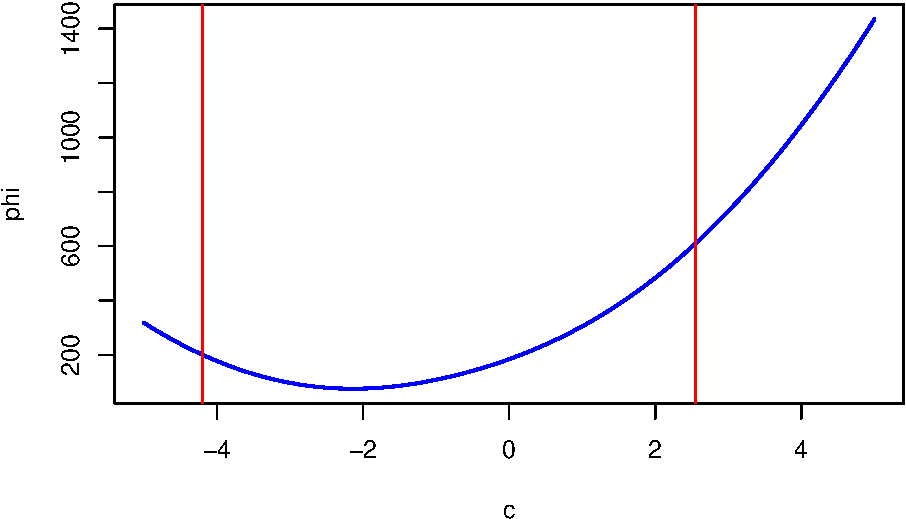
\includegraphics{smacofAC_files/figure-latex/morefunc-1.pdf}
\caption{\label{fig:morefunc}Function phi for De Gruijter example}
\end{figure}

We minimize \(\phi\) by using the R function optimize(). The minimum of \(\phi\) in our De Gruijter example turns out to be 75.251647, attained at \(c\) equal to
-2.1403321. The Shepard plot corresponding with the optimum \(c\) is plotted in figure \ref{fig:optbandplot}. Keep in mind that this is the optimal \(c\) for the initial
configuration only (and for our specific choice of bounds). As we will see in a moment the
fit can be much improved.

\begin{figure}

{\centering 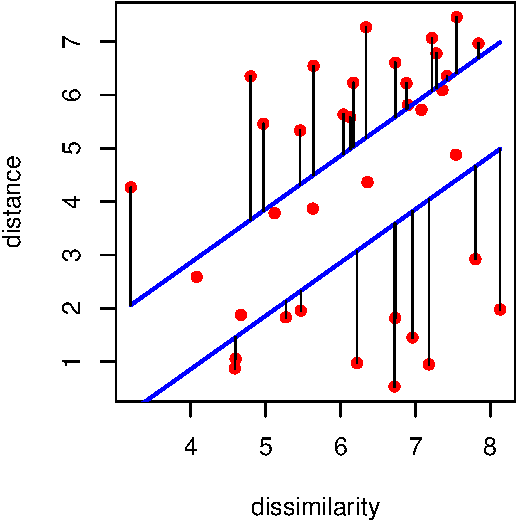
\includegraphics{smacofAC_files/figure-latex/optbandplot-1} 

}

\caption{De Gruijter Shepard Plot}\label{fig:optbandplot}
\end{figure}

\section{Example}\label{example}

In the example we again use the De Gruijter data, but now we compute optimal
solutions for all four types AC1-AC4 (two dimensions, Torgerson initial estimate,
no weights). We iterate until the difference in consecutive stress values is
less than 1e-10. For each of the four runs we give the number of iterations,
the final stress, and the additive constant in case of AC2 and AC4. We also
make three plots: the Shepard plot with points \((\delta_{ij},d_{ij}(X))\)
in blue and with points \((\delta_{ij},\hat d_{ij})\) in red, the configuration
plot with a labeled \(X\), and the dist-dhat plot with points \((d_{ij}(X),\hat d_{ij})\)
scattered around the line \(d=\hat d\). Line segments are drawn in the plots to
show the fit of all pairs \((i,j)\).

\subsection{Type AC1}\label{type-ac1-1}

For AC1 we find a minimum stress of 32.2208145 after 552 iterations.
The Shepard plot has a substantial intercept, which suggest that an additive
constant may improve the fit. This is typical for average similarity judgments
over heterogeneous groups of individuals. It is the reason why Ekman (1954)
linearly transformed his average similarities so that the smallest became zero
and the largest became one. That amounts to applying the additive constant before
the MDS analysis.

To give some content to the configuration plot: CPN (communists), PSP (pacifists),
and PvdA (social democrats) are leftists parties, ARP (protestants), CHU (other
protestants), KVP (catholics) are religious parties, BP (farmers) is a
right-wing protest party, VVD (classical liberals) is a conservative party, and D'66
(pragmatists, centrists) was brand new in 1967 and was supposedly beyond left and right.

\begin{center}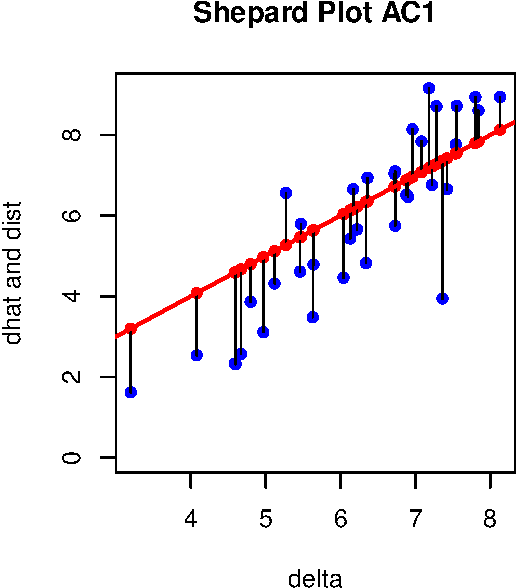
\includegraphics{smacofAC_files/figure-latex/gruijterh00-1} \end{center}

\begin{center}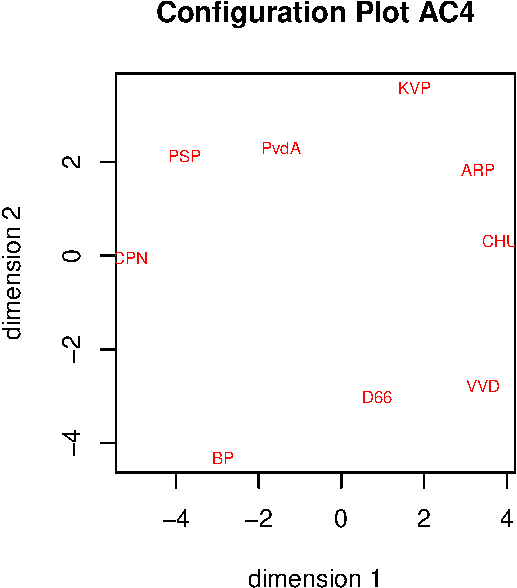
\includegraphics{smacofAC_files/figure-latex/gruijterh00-2} \end{center}

\begin{center}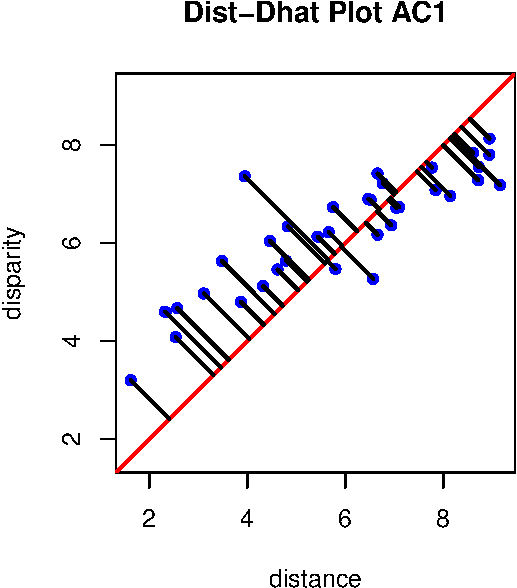
\includegraphics{smacofAC_files/figure-latex/gruijterh00-3} \end{center}

\subsection{Type AC2}\label{type-ac2-1}

As expected, the additive constant improves the fit. We have convergence after 89
iterations to stress 3.6661492. The additive constant is -3.2, which means the smallest \(\delta_{ij}+c\), between ARP and CHU, is now zero. The configuration shows the same three groups, but they cluster a bit more tightly. This is to be expected. Without the
additive constant the dissimilarities are more equal and consequently the distances are
more equal to. The configuration tends more to what we see if all dissimilarities are equal,
i.e.~to points regularly spaced on a circle (De Leeuw and Stoop (1984)).

\begin{center}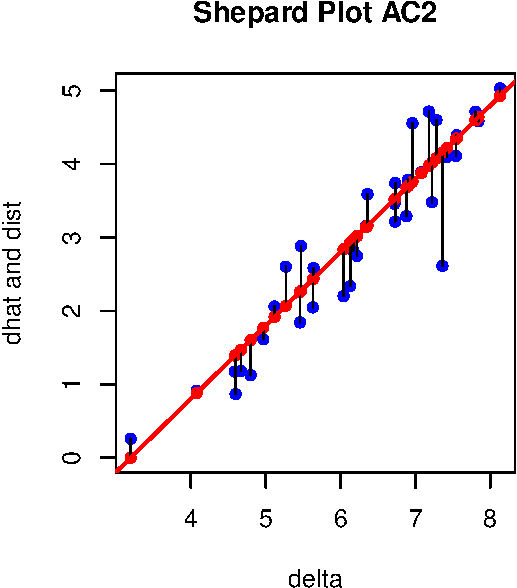
\includegraphics{smacofAC_files/figure-latex/gruijterh10-1} \end{center}

\begin{center}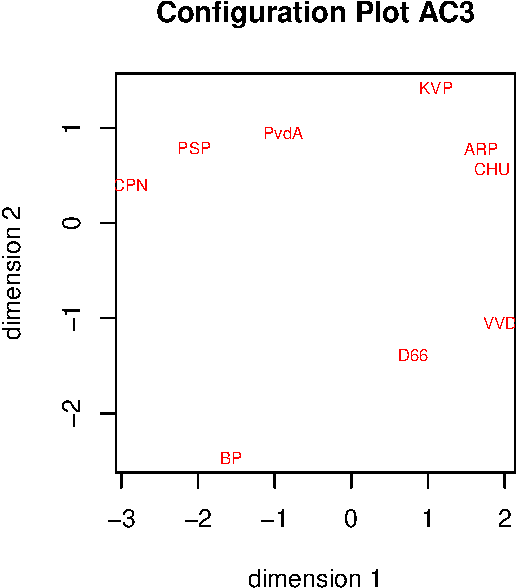
\includegraphics{smacofAC_files/figure-latex/gruijterh10-2} \end{center}

\begin{center}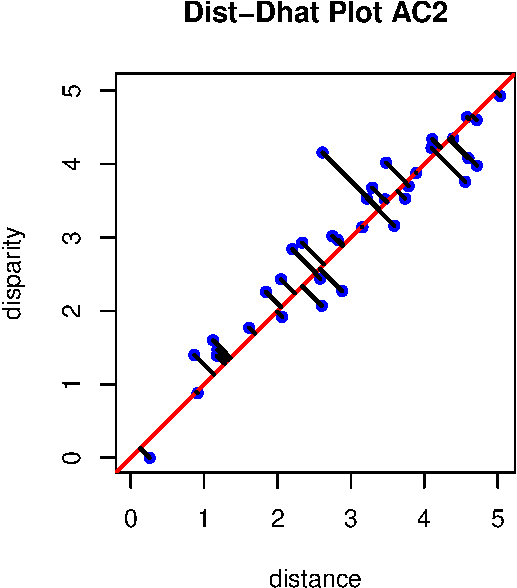
\includegraphics{smacofAC_files/figure-latex/gruijterh10-3} \end{center}

\subsection{Type AC3}\label{type-ac3-1}

The bounds we use are \(\delta_{ij}\pm 1\). After 271 iterations
we arrive at stress 5.7972. In the configuration plot the centrists
have moved to the center.

\begin{center}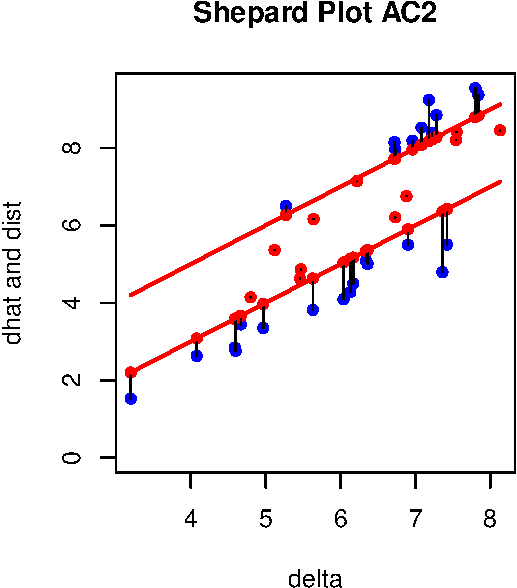
\includegraphics{smacofAC_files/figure-latex/gruijterh01-1} \end{center}

\begin{center}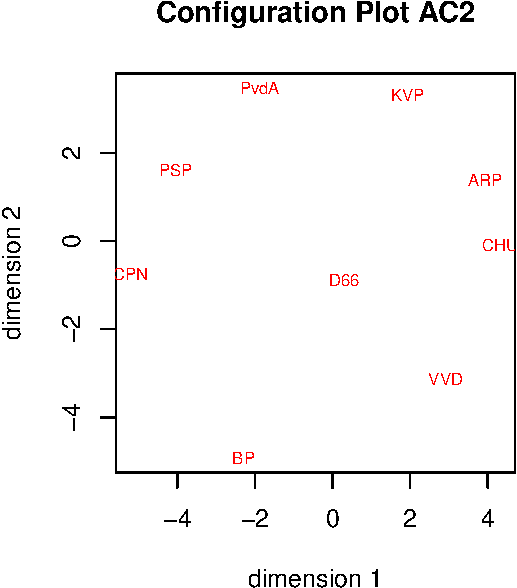
\includegraphics{smacofAC_files/figure-latex/gruijterh01-2} \end{center}

\begin{center}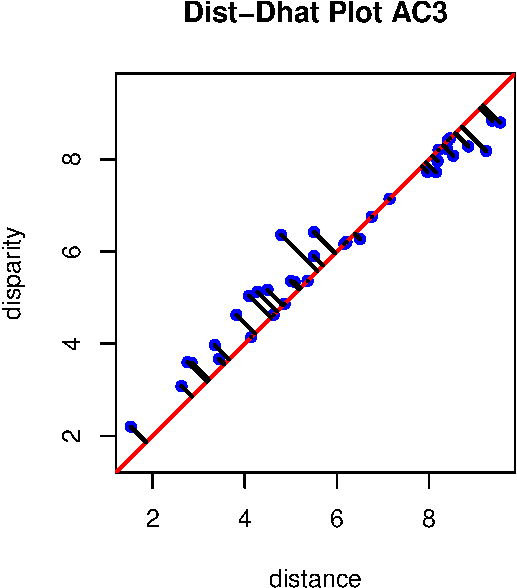
\includegraphics{smacofAC_files/figure-latex/gruijterh01-3} \end{center}

\subsection{Type AC4}\label{type-ac4-1}

After 466 iterations stress is \ensuremath{1.8821595\times 10^{-8}}, i.e.~practically zero. We succeeded in moving all distances within the bounds. The additive constant is -3.0668025. The configuration
is again pretty much the same with D'66 in the center. VVD moves closer to the Christian
Democrats, and BP is more isolated.

\begin{center}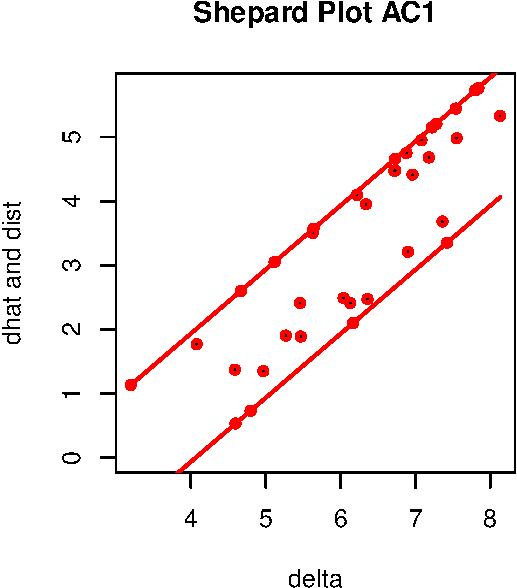
\includegraphics{smacofAC_files/figure-latex/gruijterh11-1} \end{center}

\begin{center}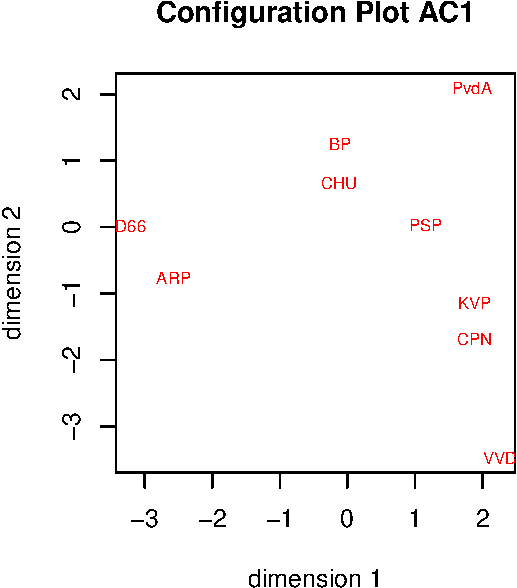
\includegraphics{smacofAC_files/figure-latex/gruijterh11-2} \end{center}

\begin{center}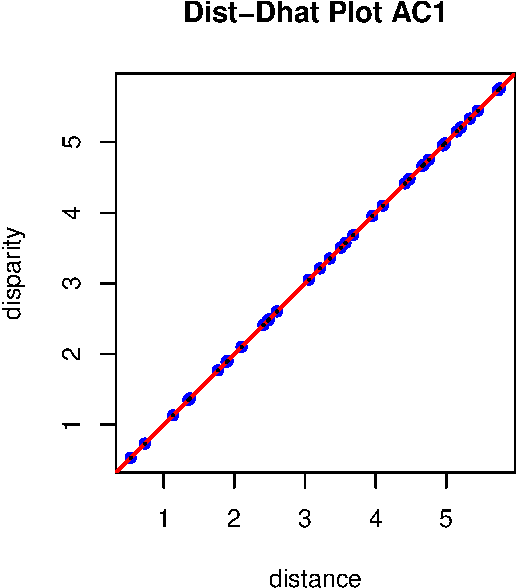
\includegraphics{smacofAC_files/figure-latex/gruijterh11-3} \end{center}

\section*{References}\label{references}
\addcontentsline{toc}{section}{References}

\phantomsection\label{refs}
\begin{CSLReferences}{1}{0}
\bibitem[\citeproctext]{ref-cooper_72}
Cooper, L. G. 1972. {``{A New Solution to the Additive Constant Problem in Metric Multidimensional Scaling}.''} \emph{Psychometrika} 37 (3): 311--22.

\bibitem[\citeproctext]{ref-degruijter_67}
De Gruijter, D. N. M. 1967. {``{The Cognitive Structure of Dutch Political Parties in 1966}.''} Report E019-67. Psychological Institute, University of Leiden.

\bibitem[\citeproctext]{ref-deleeuw_stoop_A_84}
De Leeuw, J., and I. Stoop. 1984. {``Upper Bounds for Kruskal's Stress.''} \emph{Psychometrika} 49: 391--402.

\bibitem[\citeproctext]{ref-ekman_54}
Ekman, G. 1954. {``{Dimensions of Color Vision}.''} \emph{Journal of Psychology} 38: 467--74.

\bibitem[\citeproctext]{ref-heiser_91}
Heiser, W. J. 1991. {``{A Generalized Majorization Method for Least Squares Multidimensional Scaling of Pseudodistances that May Be Negative}.''} \emph{Psychometrika} 56 (1): 7--27.

\bibitem[\citeproctext]{ref-messick_abelson_56}
Messick, S. J., and R. P. Abelson. 1956. {``{The Additive Constant Problem in Multidimensional Scaling}.''} \emph{Psychometrika} 21 (1--17).

\end{CSLReferences}

\end{document}
